\documentclass[main.tex]{subfiles}
 
\begin{document}

\section{Bus covariance}

\section{Line covariance}

By incorporating bus covariances in our model (which result from correlated weather), we hope to find new structure in the line covariances. 
To assess the effect of estimating bus covariances, we compare three possible bus covariance matrices:
\begin{enumerate}
	\item \emph{The identity matrix}: all bus injections are independently Gaussian distributed with the same variance. (They are almost IID, but their means differ.)
	\item \emph{The diagonal of estimated variances}: all bus injections are independently Gaussian distributed, but their variances and means differ.
	\item \emph{The estimated covariances}: the vector of bus injections is (multivariate) Gaussian distributed. All bus injections are, in general, dependent on each other, and their variances and means differ.
\end{enumerate}

We expect the covariance of a random pair of lines to be relatively low, when their physical separation (measured either in kilometres or in graph distance) is high. 
Because weather is correlated, even at high distance, using the bus full covariance might result in higher covariances between lines with high separation. (This was concluded by \cite{Nesti2018emergentfailures}.) 

Using a different bus covariance matrix will likely result in a overall increase or decrease of line covariances. Note, however, that the line covariance matrix is scaled by an arbitrary factor $\epsilon$, so any overall change in covariance has no significance in the model. \todo{Maar als je normaliseert op variantie?}

\towrite{Compare three bus covariance }


\begin{figure}
    \centering
    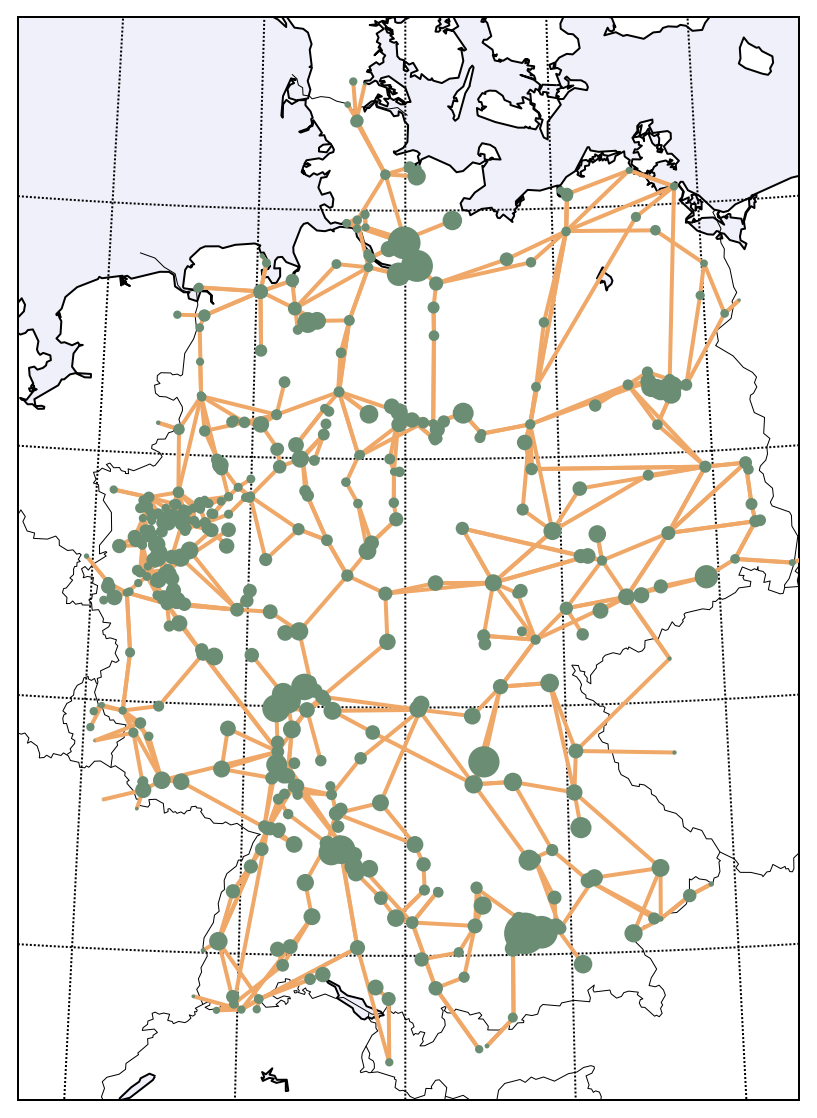
\includegraphics[width=.4\textwidth]{img/load.png}
    \caption{PLACEHOLDER: The load distribution of Germany at ???.}
    \label{fig:loaddistribution}
\end{figure}
\begin{figure}
    \centering
    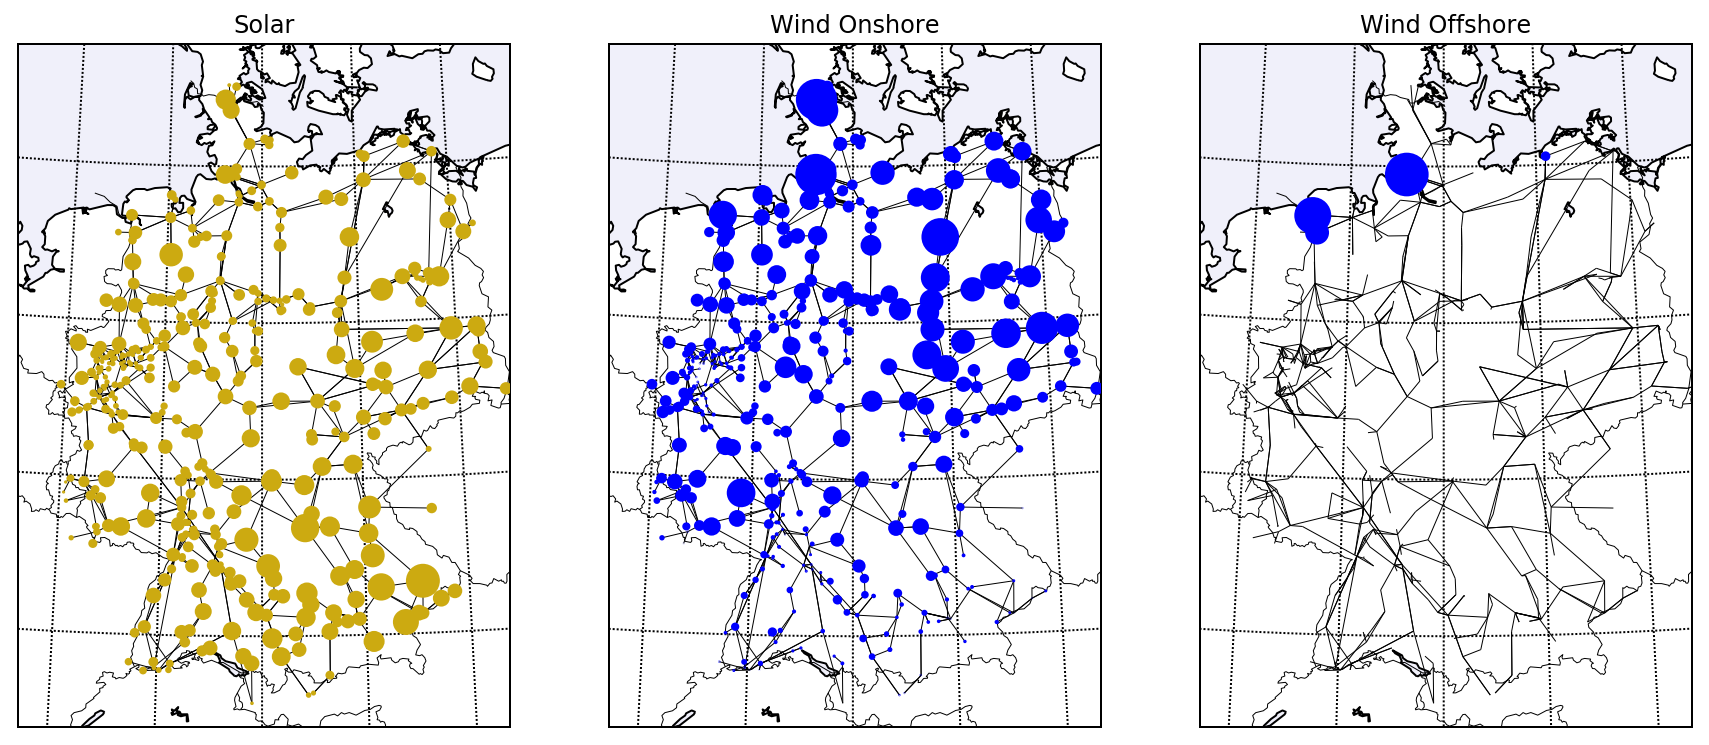
\includegraphics[width=\textwidth]{img/solarwind.png}
    \caption{PLACEHOLDER: Solar, wind onshore, wind offshore generation at ?? in Germany.}
    \label{fig:solarwind}
\end{figure}
\begin{figure}
    \centering
    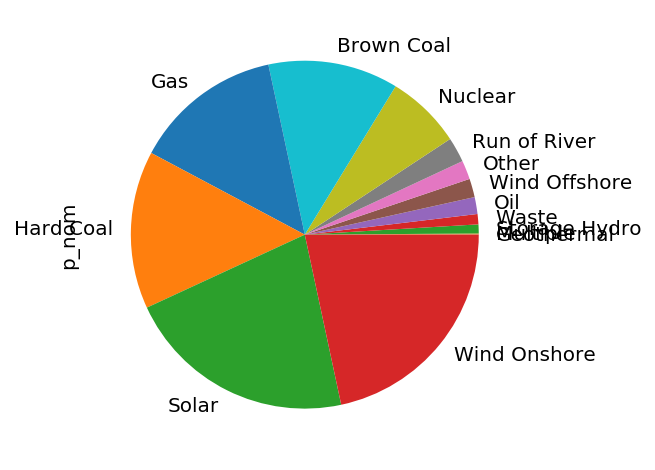
\includegraphics[width=.4\textwidth]{img/genprop.png}
    \caption{PLACEHOLDER: Generation capacity technology shares in Germany in 2011.}
    \label{fig:generationtech}
\end{figure}
\begin{figure}
    \centering
    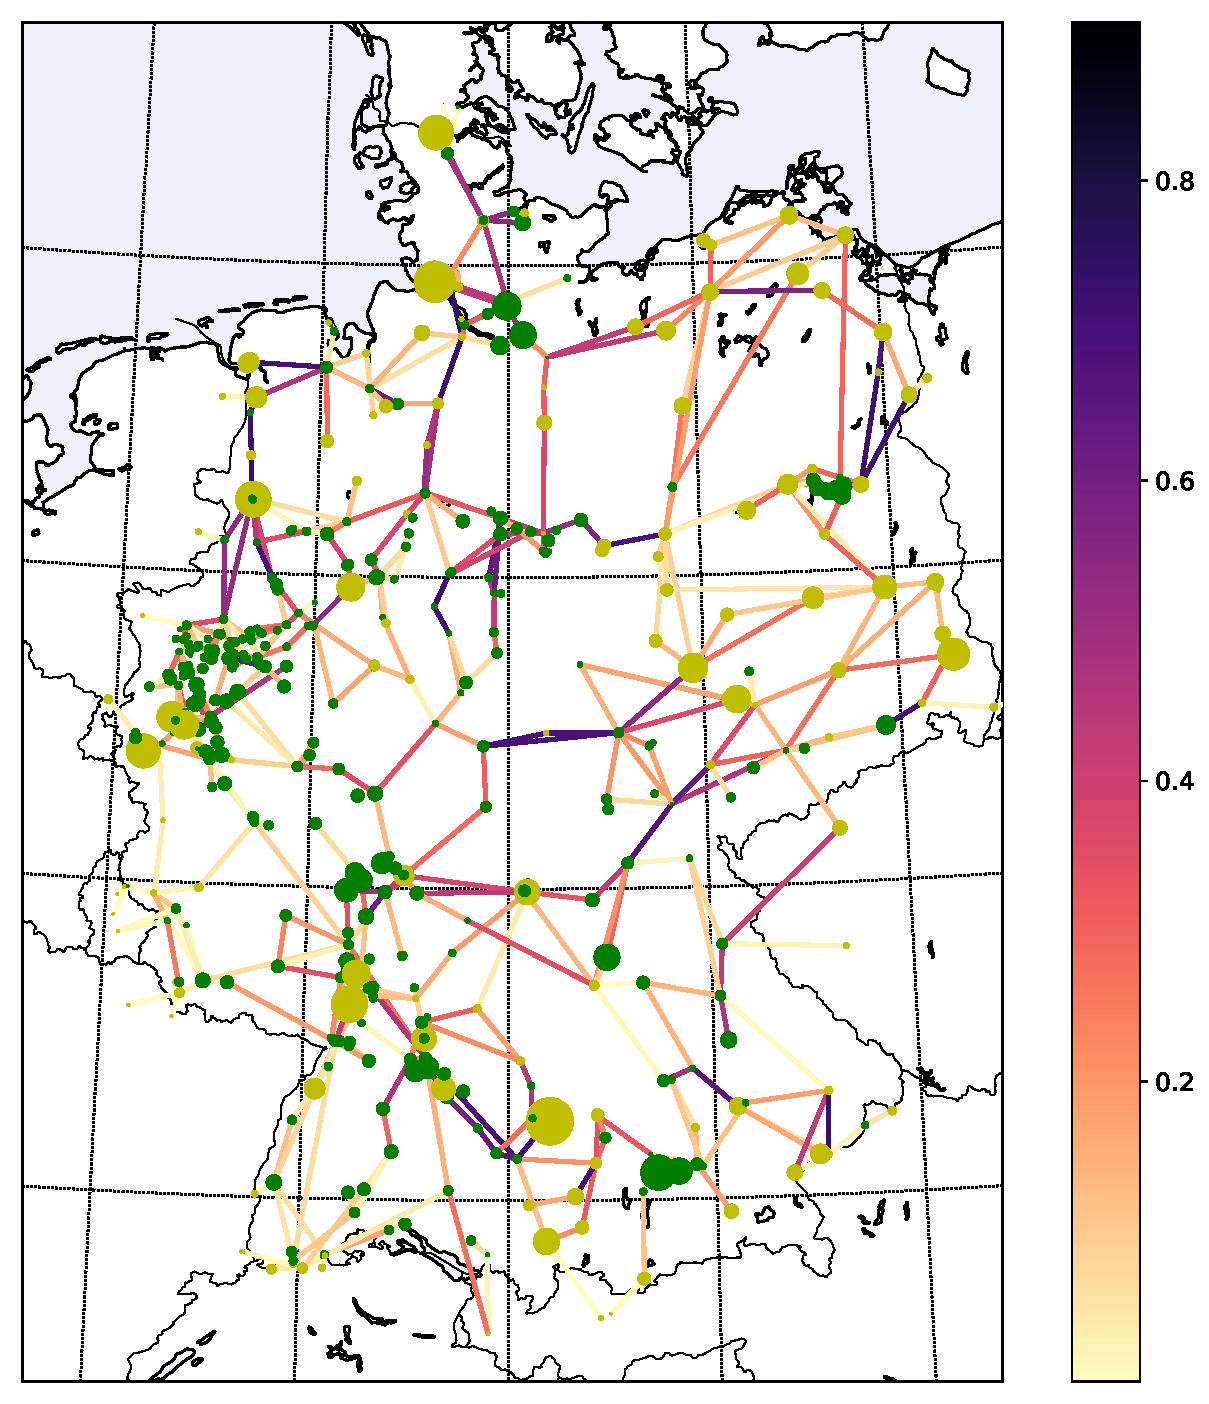
\includegraphics[width=.6\textwidth]{img/nominallineflow.pdf}
    \caption{Nominal line flow during 11:00-12:00, as fraction of line capacity. Node size represents net power injection. When generation exceeds load, the injection is positive (yellow), otherwise negative (green). \emph{Compare with Figure 1a of \cite{Nesti2018emergentfailures}.}}
    \label{fig:generationtech}
\end{figure}
asdf

\todo{Plotjes van kansen zoals in \label{stochasticpowerinjections}}

\begin{table}[]
    \centering
    \begin{tabular}{c|ccrr|ccrr}
\toprule
\multicolumn{1}{c}{} & \multicolumn{4}{c}{\textsc{Solar}} & \multicolumn{4}{c}{\textsc{Wind}} \\
\midrule
\multicolumn{1}{c}{} & 
\multicolumn{1}{c}{\textit{default}} & \multicolumn{1}{c}{\textit{modified}} & 
\multicolumn{1}{c}{1\%} & \multicolumn{1}{c}{2\%} & 
\multicolumn{1}{c}{\textit{default}} & \multicolumn{1}{c}{\textit{modified}} & 
\multicolumn{1}{c}{1\%} & \multicolumn{1}{c}{2\%} \\
\midrule
Jan & \texttt{385} & \texttt{\textbf{484}} & \texttt{\textbf{5}} & \texttt{\textbf{0}} & \texttt{\textbf{488}} & \texttt{488} & \texttt{\textbf{0}} & \texttt{\textbf{0}} \\
Feb & \texttt{364} & \texttt{\textbf{485}} & \texttt{\textbf{4}} & \texttt{\textbf{0}} & \texttt{\textbf{487}} & \texttt{487} & \texttt{\textbf{0}} & \texttt{\textbf{1}} \\
Mar & \texttt{334} & \texttt{\textbf{475}} & \texttt{\textbf{14}} & \texttt{\textbf{0}} & \texttt{\textbf{487}} & \texttt{487} & \texttt{\textbf{1}} & \texttt{\textbf{0}} \\
Apr & \texttt{211} & \texttt{\textbf{477}} & \texttt{\textbf{11}} & \texttt{\textbf{1}} & \texttt{\textbf{488}} & \texttt{488} & \texttt{\textbf{0}} & \texttt{\textbf{0}} \\
May & \texttt{189} & \texttt{\textbf{473}} & \texttt{\textbf{16}} & \texttt{\textbf{0}} & \texttt{\textbf{467}} & \texttt{467} & \texttt{\textbf{21}} & \texttt{\textbf{0}} \\
Jun & \texttt{255} & \texttt{\textbf{481}} & \texttt{\textbf{8}} & \texttt{\textbf{0}} & \texttt{\textbf{480}} & \texttt{480} & \texttt{\textbf{8}} & \texttt{\textbf{0}} \\
Jul & \texttt{292} & \texttt{\textbf{485}} & \texttt{\textbf{4}} & \texttt{\textbf{0}} & \texttt{\textbf{488}} & \texttt{488} & \texttt{\textbf{0}} & \texttt{\textbf{0}} \\
Aug & \texttt{179} & \texttt{\textbf{478}} & \texttt{\textbf{10}} & \texttt{\textbf{1}} & \texttt{\textbf{488}} & \texttt{488} & \texttt{\textbf{0}} & \texttt{\textbf{0}} \\
Sep & \texttt{259} & \texttt{\textbf{472}} & \texttt{\textbf{16}} & \texttt{\textbf{1}} & \texttt{\textbf{487}} & \texttt{487} & \texttt{\textbf{1}} & \texttt{\textbf{0}} \\
Oct & \texttt{263} & \texttt{\textbf{480}} & \texttt{\textbf{9}} & \texttt{\textbf{0}} & \texttt{\textbf{488}} & \texttt{488} & \texttt{\textbf{0}} & \texttt{\textbf{0}} \\
Nov & \texttt{290} & \texttt{\textbf{472}} & \texttt{\textbf{17}} & \texttt{\textbf{0}} & \texttt{\textbf{486}} & \texttt{486} & \texttt{\textbf{2}} & \texttt{\textbf{0}} \\
Dec & \texttt{317} & \texttt{\textbf{482}} & \texttt{\textbf{7}} & \texttt{\textbf{0}} & \texttt{\textbf{486}} & \texttt{486} & \texttt{\textbf{2}} & \texttt{\textbf{0}} \\
\bottomrule
    \end{tabular}%TODO: modified wind bold?
    \caption{Number of buses (out of 489 solar, 488 wind) for which the ARMA model could be fitted using either the \emph{default} implementation of \texttt{arima} in \texttt{R}, or the \emph{modified} version (described in \ref{arimamod}).
    \newline
    When even the modified method yielded no results, uniform noise was added to the series before fitting. Noise magnitude was set to 1\% of generation capacity, or 2\% when needed.
    \newline
    Figures in \textbf{bold} indicate which results are used.
    %All nodes now have usable results.
    }
    \label{tab:arimafitstats}
\end{table}

\begin{table}
\begin{tabular}{lll}
\toprule
$l$ & $\PROB \left[ |\mel{f}_l| \geq 1 \right]$ & $\mel{I}_l$ \\
\midrule
361 & 3.45\hphantom{0}\% &  1.65 \\
516 & 2.91\hphantom{0}\% &  1.79 \\
586 & 2.75\hphantom{0}\% &  1.84 \\
587 & 2.73\hphantom{0}\% &  1.85 \\
803 & 2.02\hphantom{0}\% &  2.10 \\
670 & 1.21\hphantom{0}\% &  2.54 \\
19  & 1.13\hphantom{0}\% &  2.60 \\
302 & 1.08\hphantom{0}\% &  2.64 \\
48  & 1.03\hphantom{0}\% &  2.68 \\
554 & 0.974\% &  2.73 \\
\midrule
488 & 0.971\% &  2.73 \\
809 & 0.824\% &  2.88 \\
28  & 0.748\% &  2.96 \\
810 & 0.728\% &  2.98 \\
29  & 0.396\% &  3.53 \\
27  & 0.355\% &  3.62 \\
389 & 0.247\% &  3.95 \\
390 & 0.245\% &  3.96 \\
486 & 0.235\% &  4.00 \\
249 & 0.056\% &  5.30 \\
\bottomrule
\end{tabular}

\caption{TODO}
\label{tab:top20}
\end{table}

\clearpage
\end{document}